\section{Overview and Implementation Plan}
\label{sec:overview_implementation}

This chapter describes the InternHub – Students \& Companies (S\&C) platform's integration strategy, test plan, and implementation procedure. A systematic and effective development process will be ensured by using the \textbf{Bottom-Up approach}.

The implementation will start with basic, independent modules that do not need additional modules to work. Drivers for testing each module separately will be created. Modules will gradually be added to the system, taking the place of their associated drivers as they are put into place and tested. For further testing, each integrated module will need its own driver.

Before a system is fully integrated, smaller functional subsystems can be created using the Bottom-Up approach. With this incremental approach:
\begin{itemize}
    \item Testing is performed on smaller parts of the system initially and continues for each module as it becomes ready, making debugging and error tracking easier.
    \item Parallel development is facilitated, allowing separate teams to work on various elements at the same time.
\end{itemize}

\section{Features Identification}
\label{sec:features_identification}

The features of the platform are prioritized based on their dependencies and importance, as outlined below:

\subsection{[F1] Login and Registration Features}
\begin{itemize}
    \item These are the core features required for students, companies, and administrators to access the platform.
    \item Include user registration, login, and secure authentication.
    \item As foundational features, they will be implemented first to support the functioning of subsequent features.
\end{itemize}

\subsection{[F2] Profile Management Features}
\begin{itemize}
    \item This set of features includes creating and managing profiles for students, companies, and administrators.
    \item Students can update personal details, upload CVs, and showcase skills.
    \item Companies can maintain organization profiles.
    \item These features serve as the foundation for the search and application functionalities.
\end{itemize}

\subsection{[F3] Internship Management Features}
\begin{itemize}
    \item Includes the ability for companies to create, update, and delete internship postings.
    \item Involves managing applications received for these internships.
    \item Requires proper implementation of profile management ([F2]).
    \item Will be developed subsequently after [F1] and [F2].
\end{itemize}

\subsection{[F4] Search and Filter Features}
\begin{itemize}
    \item This includes submitting applications, reviewing them, scheduling interviews, and notifying users about interview updates.
    
    \item These features depend on the successful implementation of profile and internship management ([F2] and [F3]).
\end{itemize}

\subsection{[F5] Application and Interview Features}
\begin{itemize}
    \item Includes submitting applications, reviewing them, scheduling interviews, and notifying users about interview updates.
    \item These features depend on internship management ([F3]) and profile management ([F2]).
\end{itemize}

\subsection{[F6] Complaint Handling Features}
\begin{itemize}
    \item Allows students and companies to lodge complaints and administrators to review and resolve them.
    \item Ensures user satisfaction and platform reliability.
    \item Relies on the proper implementation of profile management ([F2]) and dashboard functionalities ([F8]).
\end{itemize}

\subsection{[F7] Notification Features}
\begin{itemize}
    \item Ensure that students, companies, and administrators are notified about critical events such as interview schedules, application updates, and complaint resolutions.
    \item These features will be developed last as they depend on the correct functioning of all other features.
\end{itemize}

\subsection{[F8] Dashboard Features}
\begin{itemize}
    \item The dashboard provides an overview of active internships, applications, interviews, and platform activities for students, companies, and administrators.
    \item Consolidates data from various modules.
    \item Critical for system usability.
\end{itemize}

\subsection{Development Dependencies}
\label{subsec:development_dependencies}

The dependencies between the features ensure a structured and incremental implementation:
\begin{enumerate}
    \item [F1] Login and Registration Features serve as the foundation for all other functionalities.
    \item [F2] Profile Management Features are prerequisites for Internship Management ([F3]) and Search and Filter ([F4]).
    \item [F3] Internship Management Features depend on Profile Management ([F2]) and support Application and Interview Features ([F5]).
    \item [F4] Search and Filter Features depend on both Profile Management ([F2]) and Internship Management ([F3]).
    \item [F5] Application and Interview Features depend on Profile Management ([F2]), Internship Management ([F3]), and Search and Filter ([F4]).
    \item [F6] Complaint Handling Features rely on Profile Management ([F2]) and Dashboard Features ([F8]).
    \item [F7] Notification Features depend on the correct functioning of all other features.
    \item [F8] Dashboard Features consolidate data from all modules and rely on their successful implementation.
\end{enumerate}

This dependency-based plan ensures that features are developed systematically, reducing errors and facilitating incremental testing.

\section{Implementation Strategy}
\label{subsec:implementation_strategy}

\subsection{Overview and Integration Plan}
\label{subsubsec:integration_plan}

A systematic \textbf{bottom-up method} is used to integrate the system's components. The emphasis will be on developing solid foundational modules that can be gradually combined, starting with the essential elements. Before each module is integrated into the larger system, it will be tested using the relevant drivers. This approach enables:
\begin{itemize}
    \item Parallel programming.
    \item Effective debugging.
    \item Incremental functional validation.
\end{itemize}

The following crucial areas will be included in the integration process:

\paragraph{Core Model Integration}

The core model integration, which includes the data models necessary for the platform's operation, serves as the system's cornerstone. These include:
\begin{itemize}
    \item \textbf{User Model:} Manages user-related information.
    \item \textbf{Resume Model:} Handles CVs and profile details.
    \item \textbf{Internship Model:} Stores internship data.
    \item \textbf{Application Model:} Tracks internship applications.
    \item \textbf{Interview Model:} Manages interview scheduling and feedback.
    \item \textbf{Complaint Model:} Logs and tracks complaints.
\end{itemize}
\begin{figure}[H]
    \begin{center}
        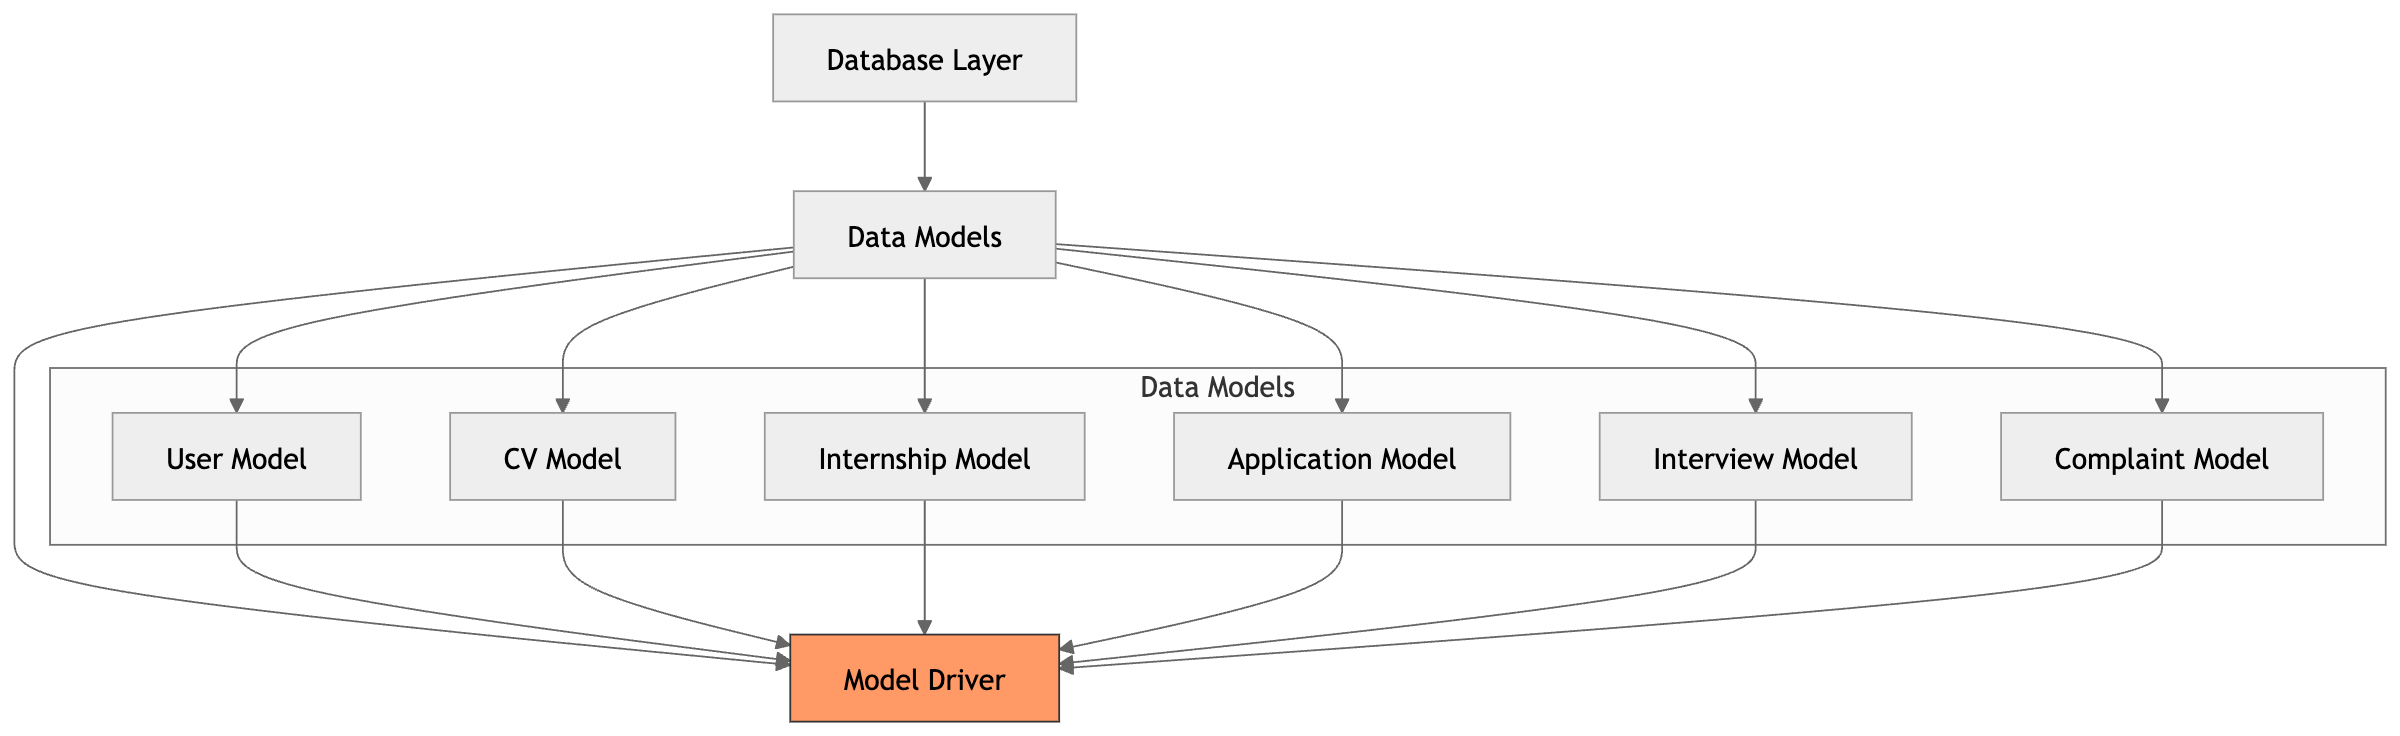
\includegraphics[width=0.79\linewidth]{JhaBhatiaSharma/imagesDD/CoreModelIntegration.png}
        \caption{Core Model Integration}
        \label{fig:coreModelIntegration}
    \end{center}
\end{figure}
In order to carry out CRUD activities and guarantee data consistency and integrity, each of these data models communicates with the database layer. To test each of these models separately and confirm that they can manage database layer interactions efficiently, a Model Driver will be put in place. These models will be incorporated into the corresponding manager components after they have been validated.

\paragraph{Authentication Integration}

The procedures involved in user registration and login are the main focus of the authentication integration. Interactions between the data models and the user interfaces for registration and login will be managed by the \textbf{Authentication Manager}. Key functionalities include:
\begin{itemize}
    \item Secure communication with the Registration System.
    \item Data validation.
    \item Access token generation.
    \item Credential validation workflows.
\end{itemize}
\begin{figure}[H]
    \begin{center} 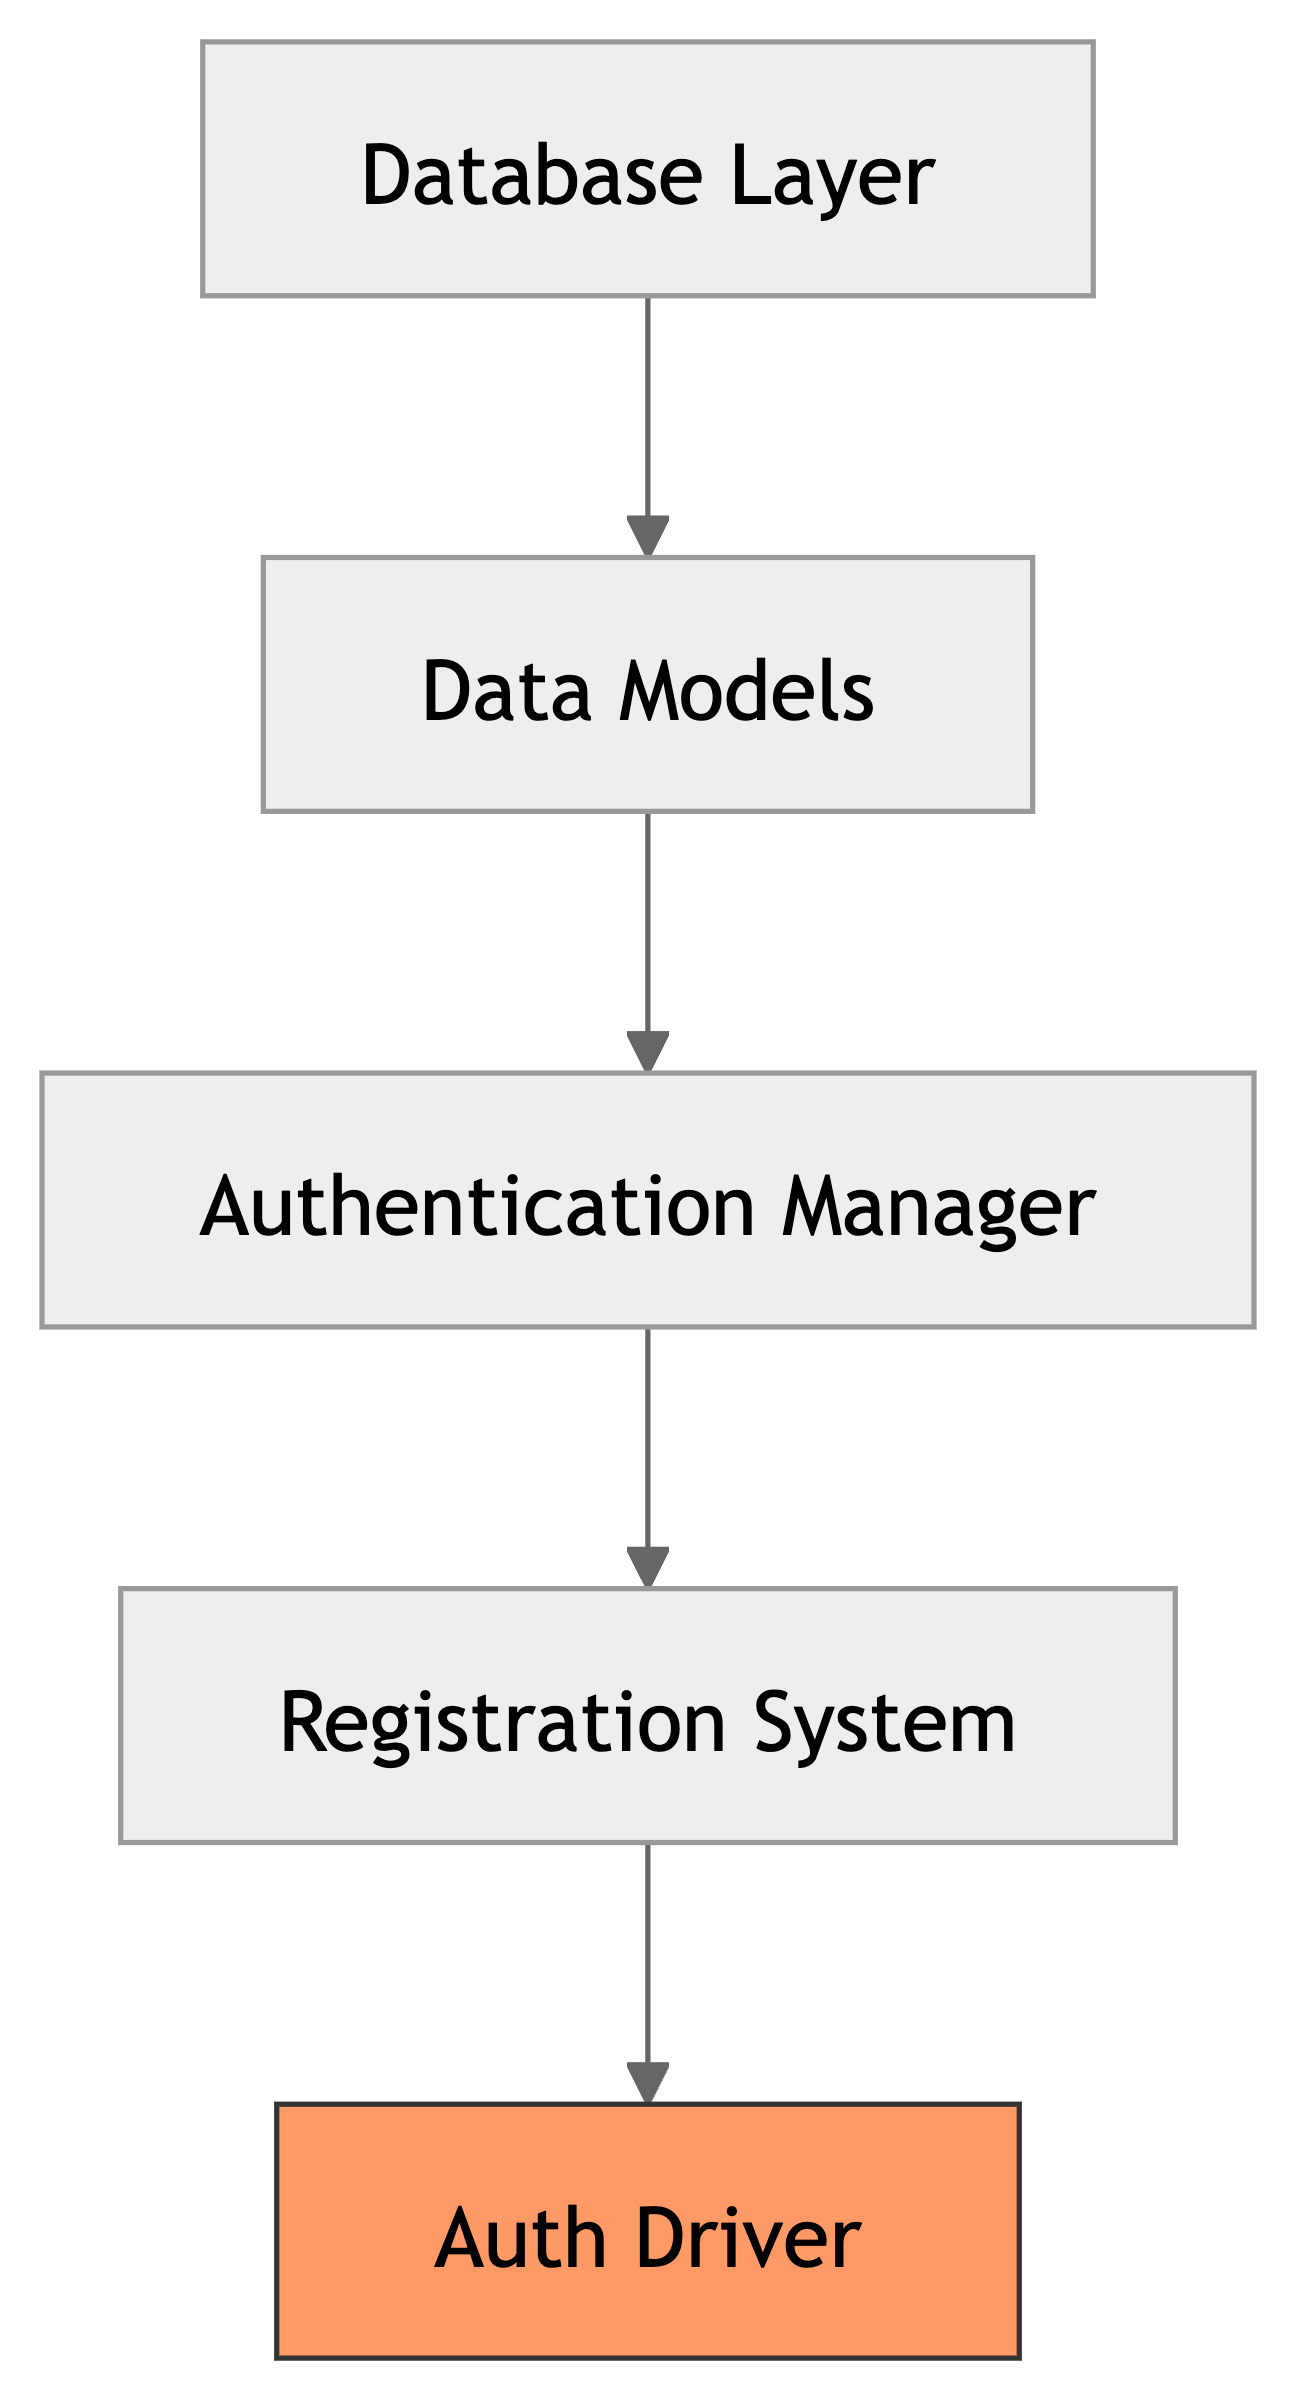
\includegraphics[width=0.18\linewidth]{JhaBhatiaSharma/imagesDD/AuthenticationIntegration.png}
    \caption{Authentication Integration}
        \label{fig:authenticationIntegration}
    \end{center}
\end{figure}

Workflows for authentication, such as the creation of access tokens and credential validation, will be tested using a driver. The Authentication Manager will be connected with the larger system to facilitate user authentication and smooth login once it is stable.


\paragraph{Profile Management Integration}
The \textbf{Profile Manager}, which manages the creation and administration of admin, company, and student profiles, is implemented as part of the Profile Management Integration. To guarantee that only authorized users are able to manage their profiles, this module communicates directly with the Authentication Manager. Key features include:
\begin{itemize}
    \item Profile creation.
    \item Profile editing.
    \item Profile retrieval.
\end{itemize}
\begin{figure}[H]
    \begin{center}
        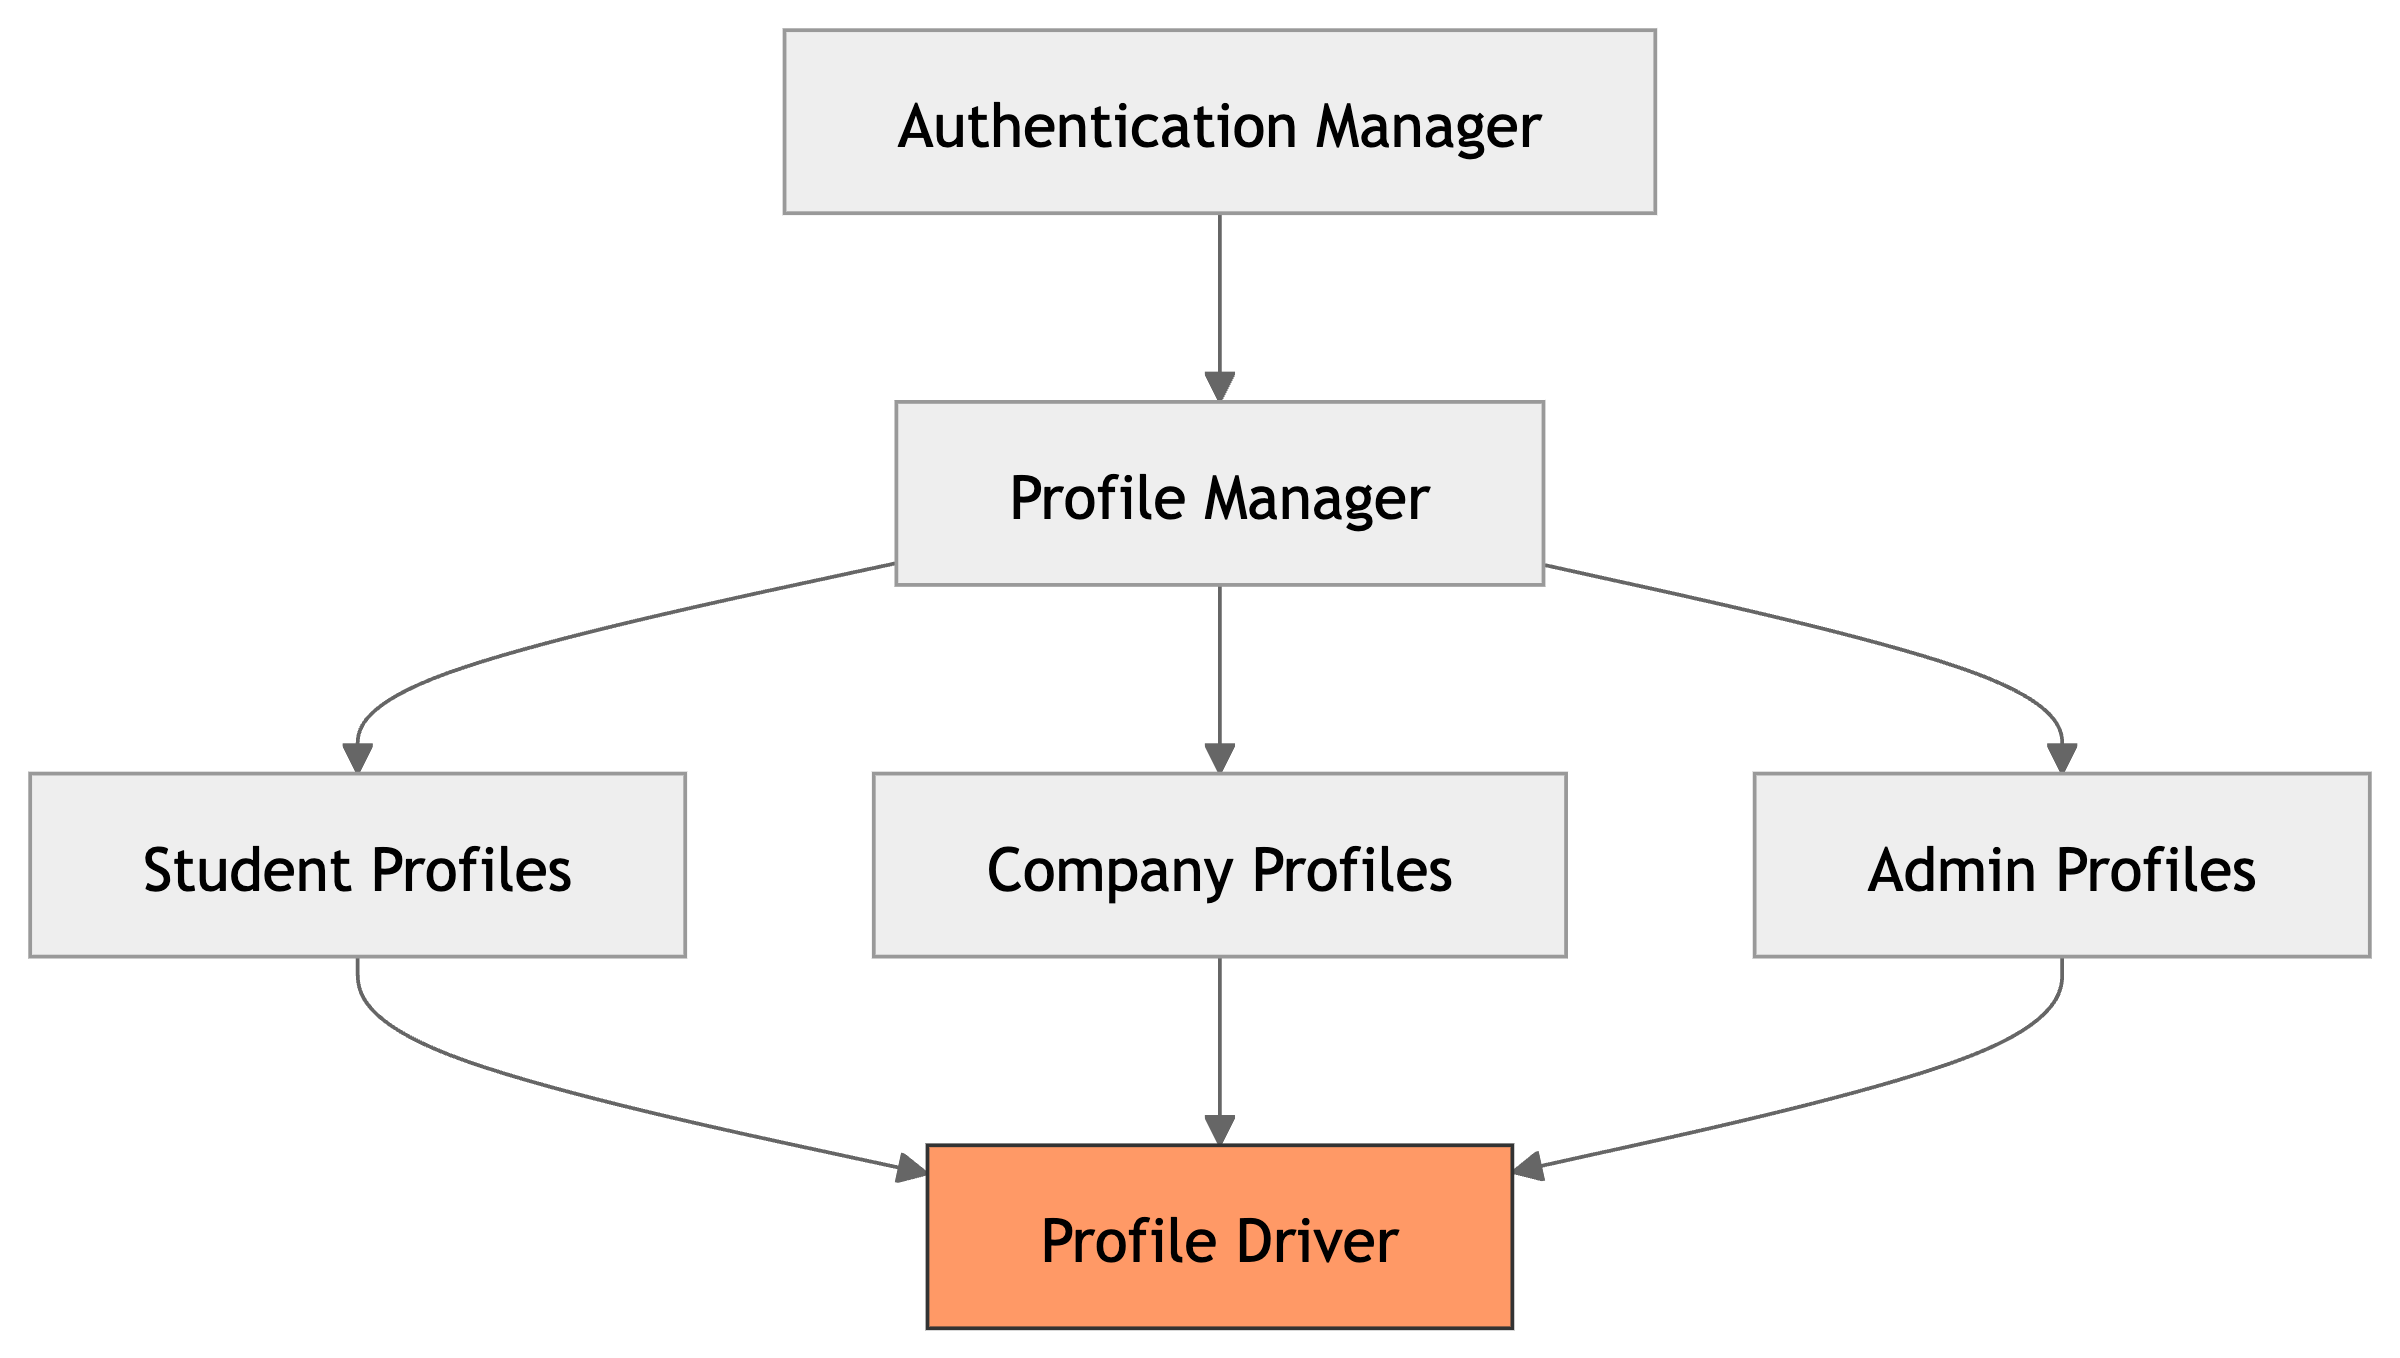
\includegraphics[width=0.79\linewidth]{JhaBhatiaSharma/imagesDD/ProfileIntegration.png}
        \caption{Profile Management Integration}
        \label{fig:profileManagement}
    \end{center}
\end{figure}
The \textbf{Profile Driver} will test these features to validate functionality. This integration is critical for enabling personalized user experiences and creating user identification across the platform.

\paragraph{Internship Management Integration}

The \textbf{Internship Manager} is at the center of the Internship Management Integration, coordinating the posting and administration of internship opportunities. It integrates with:
\begin{itemize}
    \item The Profile Manager to verify recruiter responsibilities and permissions.
    \item The Application System to manage student applications and facilitate filtering and internship searches.
\end{itemize}
\begin{figure}[H]
    \begin{center}
        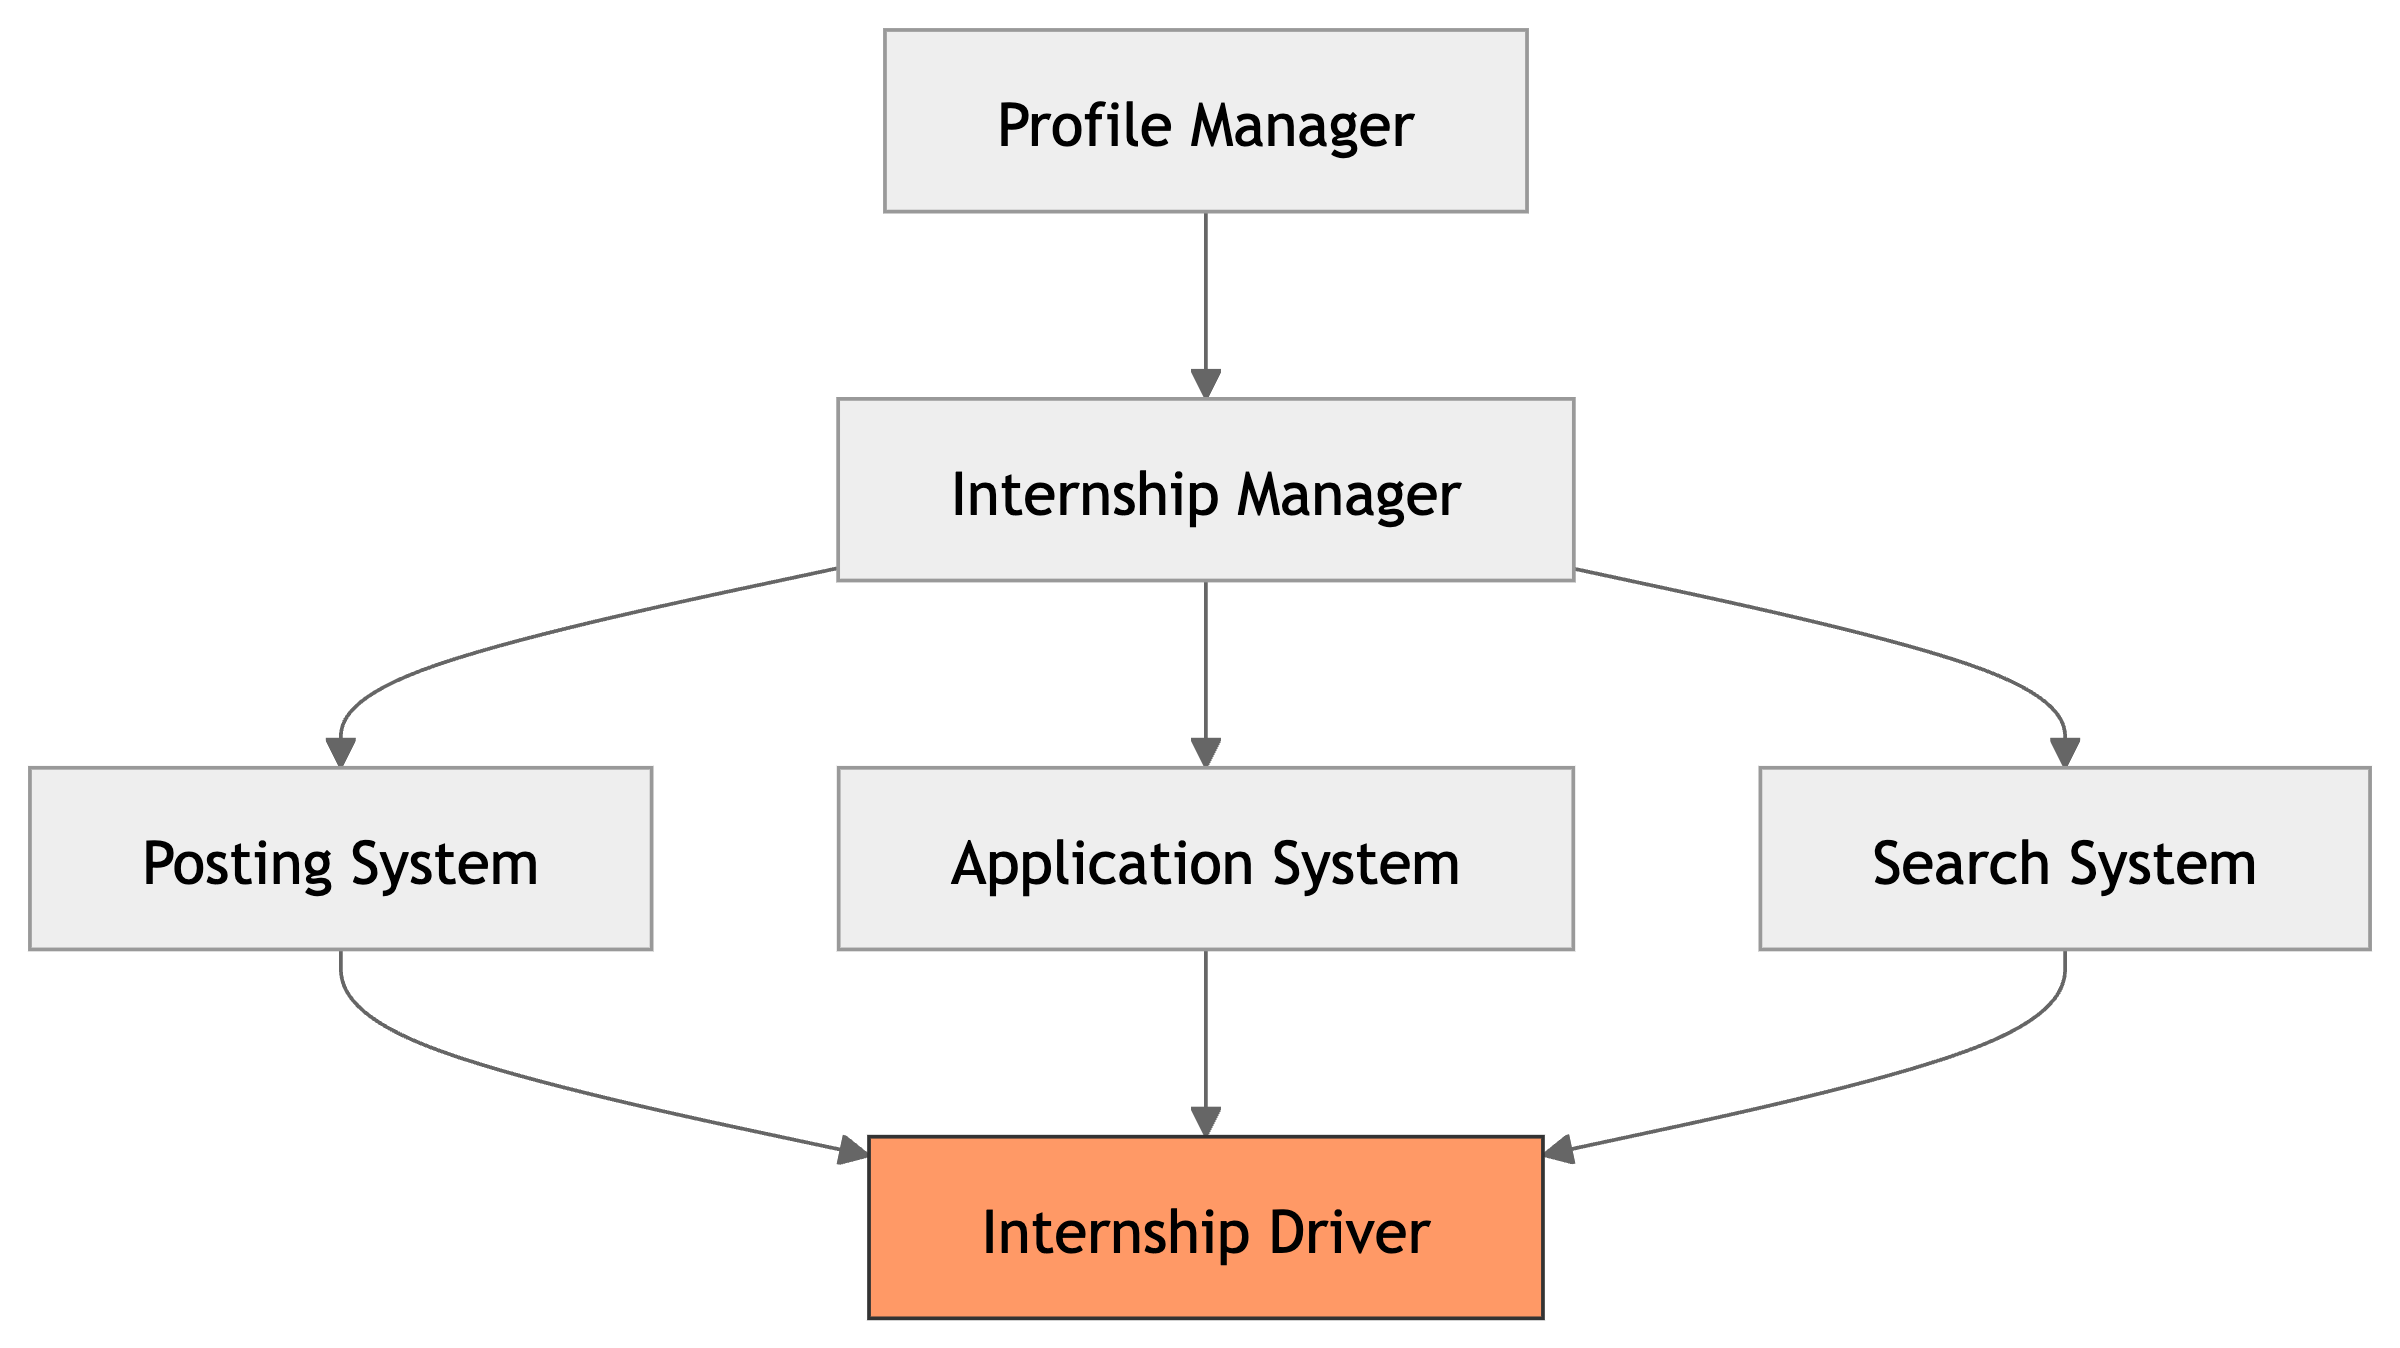
\includegraphics[width=0.79\linewidth]{JhaBhatiaSharma/imagesDD/InternshipManagementIntegration.png}
        \caption{Internship Management Integration}
        \label{fig:internshipManagement}
    \end{center}
\end{figure}
A driver will test functionalities such as posting, deleting, and searching for internships to ensure safe and effective internship management.

\paragraph{Interview and Communication Integration}
The \textbf{Interview Manager} and \textbf{Communication Manager} are responsible for interview scheduling and stakeholder communication. The integration includes:
\begin{itemize}
    \item The Scheduling System to handle interview setups.
    \item The Feedback System to collect post-interview feedback.
\end{itemize}
\begin{figure}[H]
    \begin{center}
        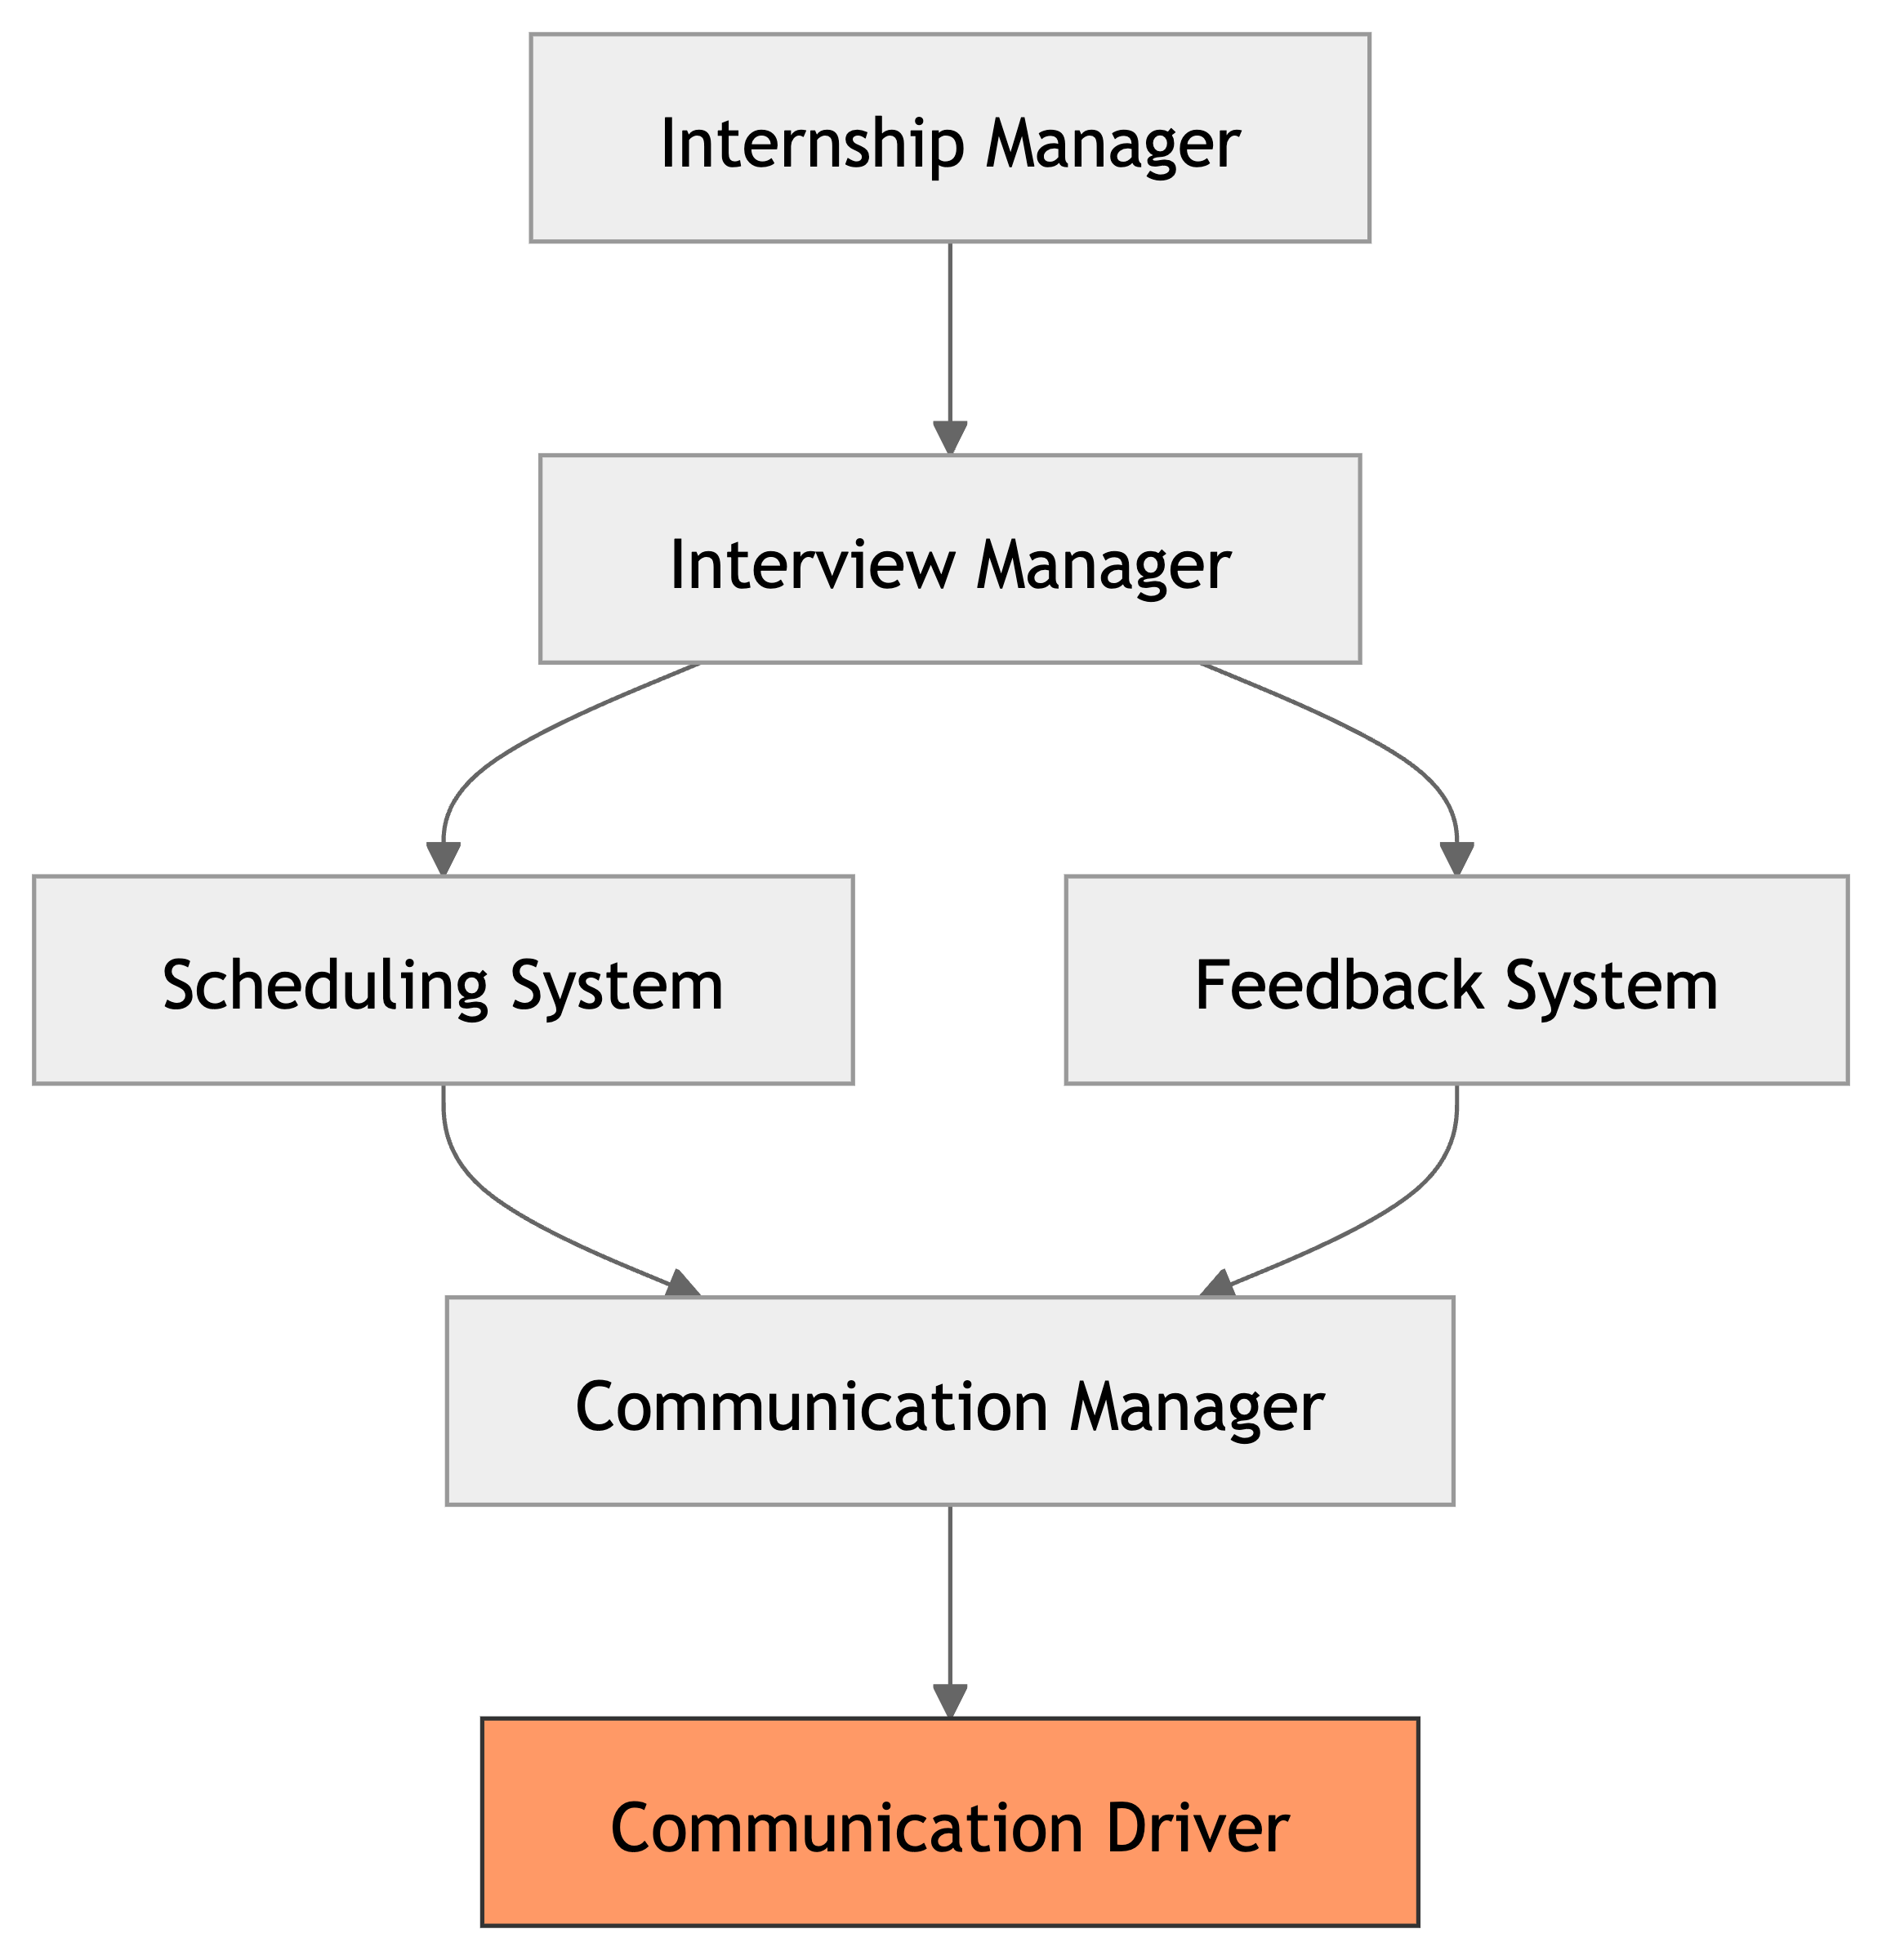
\includegraphics[width=0.59\linewidth]{JhaBhatiaSharma/imagesDD/InterviewandCommunicationIntegration.png}
        \caption{Internship and Communication Integration}
        \label{fig:internshipManagement}
    \end{center}
\end{figure}
The Communication Manager oversees the coordination of these systems, guaranteeing smooth communications and notifications. The integration of these elements will be tested by a Communication Driver, which will confirm that information is flowing between the user interface and interview management.


\paragraph{Administrative Features Integration}
The \textbf{Admin Manager} is integrated with the following systems:
\begin{itemize}
    \item Monitoring System.
    \item Reporting System.
    \item Complaint System.
\end{itemize}
\begin{figure}[H]
    \begin{center}
      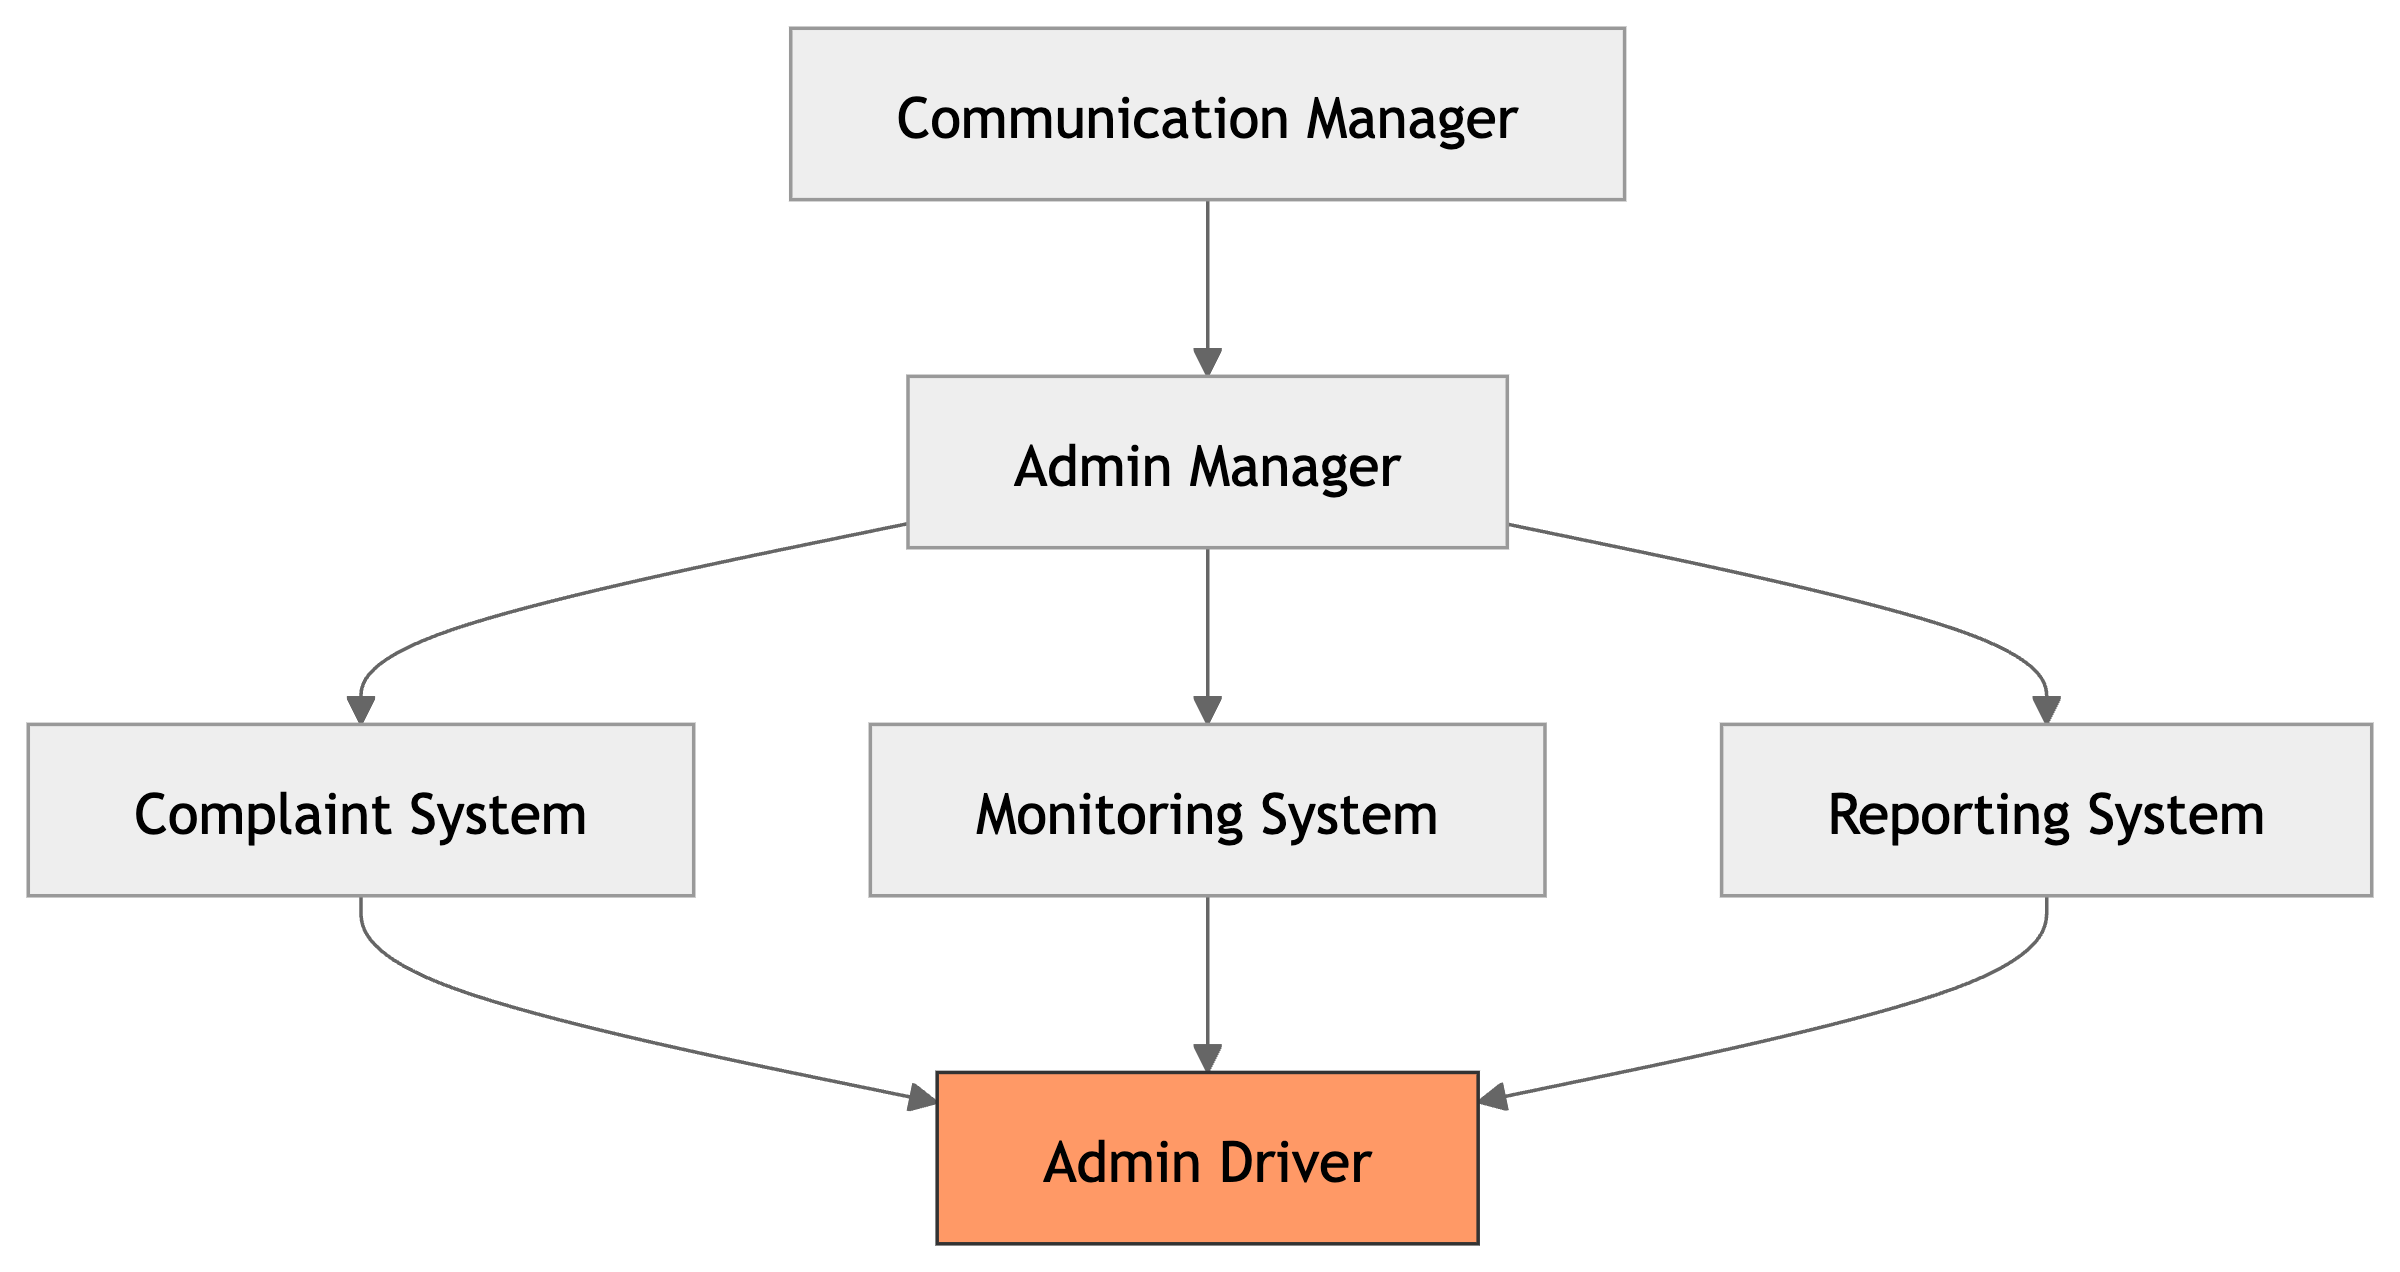
\includegraphics[width=0.59\linewidth]{JhaBhatiaSharma/imagesDD/AdministrativeFeaturesIntegration.png}
        \caption{Administrative Features Integration}
        \label{fig:adminstrativefeatures}
    \end{center}
\end{figure}
This integration also includes the Communication Manager to provide efficient communication for administrative duties. Functionalities like managing complaints, keeping an eye on platform activity, and producing reports are tested using the Admin Driver. This guarantees the stability and effectiveness of the platform's administrative functions.


\paragraph{Final System Integration}
All of the primary managers—Authentication Manager, Profile Manager, Internship Manager, Interview Manager, Communication Manager, and Admin Manager—must be connected to the \textbf{Dashboard Manager} as part of the last integration. This integration ensures:
\begin{itemize}
    \item Seamless coordination of data and processes across the platform.
    \item A unified user experience.
\end{itemize}
\begin{figure}[H]
    \begin{center}
      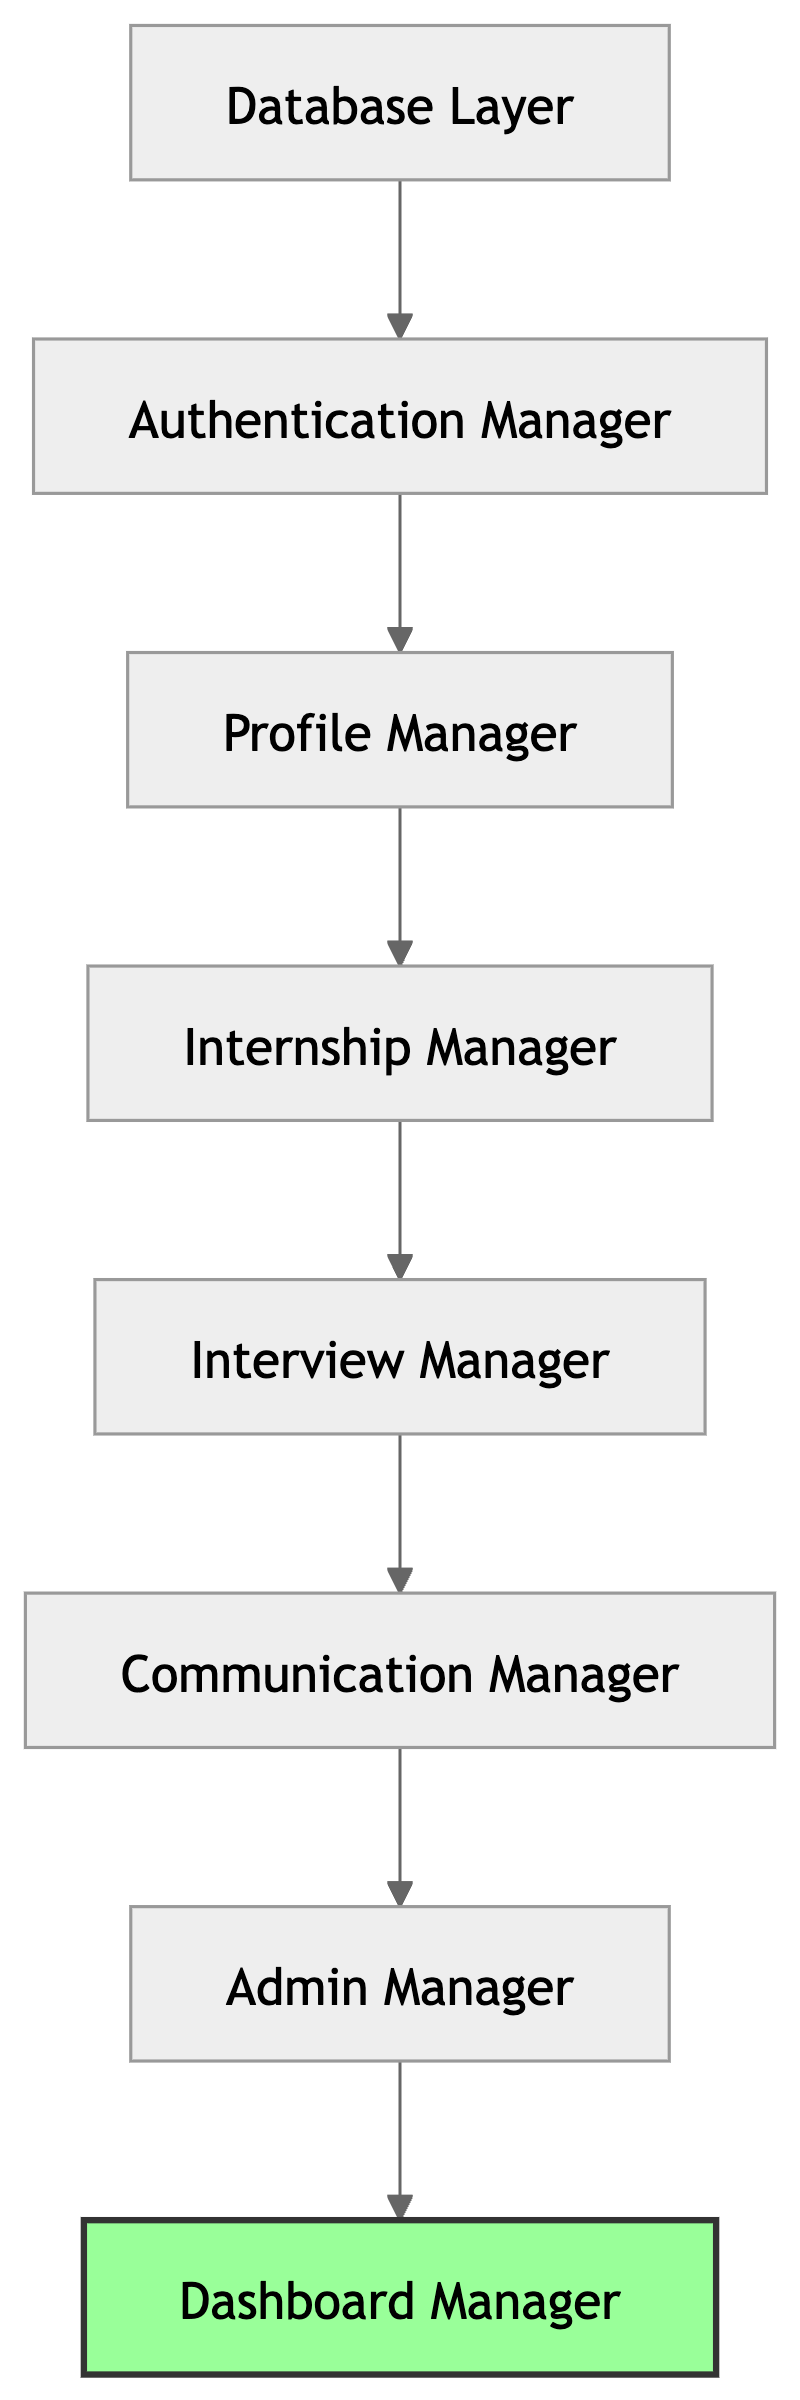
\includegraphics[width=0.18\linewidth]{JhaBhatiaSharma/imagesDD/FinalSystemIntegration.png}
        \caption{Final System Integration}
        \label{fig:finalsystemintegration}
    \end{center}
\end{figure}

Coordinating data and system processes, the Dashboard Manager acts as the main interface. With this phase, the integration process is complete, and the platform is completely functional and easy to use.
\section{System Testing Strategy}
\label{sec:system_testing_strategy}

Every newly created component will go through extensive testing before being incorporated into the system in order to guarantee the platform's accuracy and dependability. To verify each component's unique functionality, drivers will be used. To make sure that module properties are maintained and the workflow as a whole is unaffected, a new driver will be utilized to test the new component's compatibility with the current system after integration. Testing of the entire system will be done once all the components have been integrated to ensure correct operation and the lack of flaws. The testing methods listed below will be used:


\subsection{Functional Testing}
Functional testing will confirm that all objectives, specifications, and use cases are satisfied and that the platform complies with the capabilities described in the RASD document. This testing will check expected results by simulating user scenarios and confirming the system's proper workflow. Key elements that will be tested include:
\begin{itemize}
    \item Applications
    \item Internship postings
    \item Profile management
    \item Login
    \item Interview scheduling
    \item Complaint handling
\end{itemize}

\subsection{Load Testing}
The system's behavior under various workloads will be evaluated through load testing to identify:
\begin{itemize}
    \item Memory leaks
    \item Buffer overflows
    \item Inefficient memory management
\end{itemize}
This testing is necessary to confirm that the platform can efficiently manage several requests at once and remains stable during periods of high user activity.

\subsection{Performance Testing}
Performance testing will identify bottlenecks and assess how quickly the system responds to demanding workloads. This ensures that:
\begin{itemize}
    \item The platform supports many users concurrently with minimal latency.
    \item Optimization opportunities in the underlying algorithms are identified to improve overall system performance.
\end{itemize}

\subsection{Stress Testing}
To make sure the system can bounce back from errors, stress testing will mimic harsh scenarios like a large number of people using the system at once or a reduction in processing power. Through this testing, the platform's robustness and resilience will be confirmed, guaranteeing that users will experience the least amount of disturbance possible in emergency situations.


\subsection{User Interface Testing}
User interface testing will validate the platform's usability and accessibility across a variety of devices and browsers. This testing will:
\begin{itemize}
    \item Ensure a smooth and uniform experience for all user types—students, companies, and administrators.
    \item Verify compatibility with various screen sizes and resolutions.
\end{itemize}

\subsection{Comprehensive Testing Approach}
The system's functionality, reliability, and scalability will be fully verified by combining the following testing techniques:
\begin{itemize}
    \item Functional Testing
    \item Load Testing
    \item Performance Testing
    \item Stress Testing
    \item User Interface Testing
\end{itemize}
This comprehensive approach guarantees:
\begin{itemize}
    \item A flawless user experience.
    \item Compliance with the specifications outlined in the RASD document.
\end{itemize}
